%Start
%
%
%******************************************************************************************************%
%                                            Mohr's circle                                             %
%******************************************************************************************************%
% Draws Mohr's circle for given stress - values before and after rotation.                             %
% Inputs are the stress - values and the angle of rotation                                             %
%******************************************************************************************************%
% Version 1,                                                                                           %
% 29.07.2023                                                                                           %
% L.Lentz@umwelt-campus.de                                                                             %
%******************************************************************************************************%
%
\documentclass[tikz,border=10pt]{standalone}
\usetikzlibrary{calc}
%
\tikzset{
prerot/.style = {line width = 1.5pt, color = gray},
postrot/.style = {line width = 1.5pt, color = red},
reflineprerot/.style = {line width = 1.pt,  color = gray, dashed},
reflinepostrot/.style = {line width = 1.pt,  color = black, dashed}}
%
\begin{document}
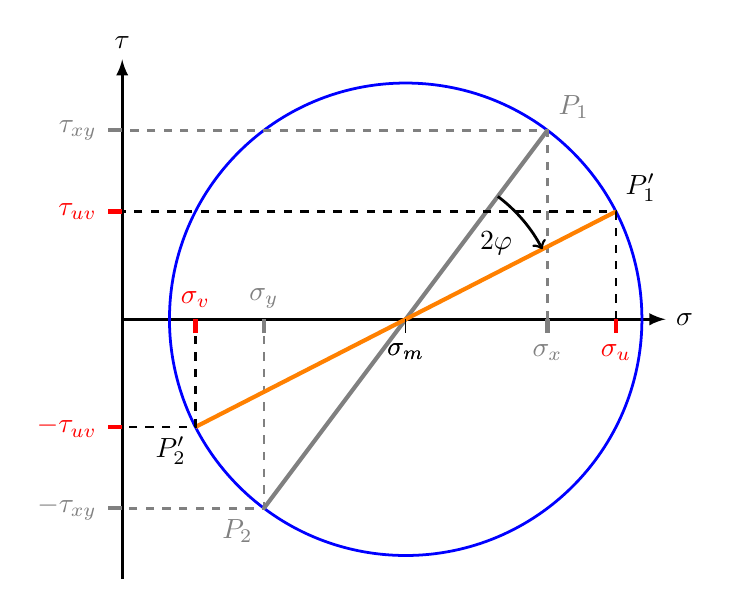
\begin{tikzpicture}[scale=0.6]
%
%
%''''''''''''''''''''''''''''Choose stress values''''''''''''''''''''''''''''''''''''''''''''''''''''''''
\def\sigmax{9} % upper normal-stress value before rotation
\def\sigmay{3} % lower normal-stress value before rotation
\def\tauxy{4} % shear-stress value before rotation
%
\def\phi{13} % angle for rotation
%''''''''''''''''''''''''''''''''''''''''''''''''''''''''''''''''''''''''''''''''''''''''''''''''''''''''
%
\pgfmathsetmacro\sigmam{0.5*(\sigmax+\sigmay)} % compute center of circle
\pgfmathsetmacro\sigmad{0.5*(\sigmax-\sigmay)} % compute x-component of radius
\pgfmathsetmacro\r{sqrt((\sigmad)^2+\tauxy^2)} % compute radius of circle
%
\pgfmathsetmacro\sigmau{\sigmam+\sigmad*cos(2*\phi)+\tauxy*sin(2*\phi)} % compute upper normal-stress value after rotation
\pgfmathsetmacro\sigmav{\sigmam-\sigmad*cos(2*\phi)-\tauxy*sin(2*\phi)} % compute lower normal-stress value after rotation
\pgfmathsetmacro\tauuv{-\sigmad*sin(2*\phi)+\tauxy*cos(2*\phi)} % compute shear-stress value after rotation
%
\def\s{0.5} % parameter for small offsets
\pgfmathsetmacro\w{\sigmam+\r+\s} % parameter for width
\pgfmathsetmacro\h{\r+\s} % parameter for heigth
%
%\draw[step=0.5,gray] (-4*\s,-\h) grid (\w+\s,\h+\s);% turn on grid if wanted
%
% coordinate system
\draw[line width = 1pt,-latex](0,-\h)--(0,\h)node[at end, anchor = south]{$\tau$};
\draw[line width = 1pt,-latex](0,0)--(\w,0)node[at end, anchor = west]{$\sigma$};
%
%draw circle
\draw[color = blue, line width = 1pt](\sigmam,0) circle (\r);
%
%----------------------------------------------------------------------------------
% draw system before rotation
%
% draw connecting line
\draw[prerot](\sigmax,\tauxy)--(\sigmay,-\tauxy);
\node at (\sigmax,\tauxy)[anchor=south west, prerot]{$P_1$};
\node at (\sigmay,-\tauxy)[anchor=north east, prerot]{$P_2$};
%
% draw stress values
\draw[reflineprerot](\sigmax,0)--+(0,\tauxy)--(0,\tauxy);
\draw[reflineprerot](\sigmay,0)--+(0,-\tauxy)--(0,-\tauxy);
\draw[prerot](0,\tauxy)--+(-0.3,0)node[anchor = east]{$\tau_{xy}$};
\draw[prerot](0,-\tauxy)--+(-0.3,0)node[anchor = east]{$-\tau_{xy}$};
\draw[prerot](\sigmax,0)--+(0,-0.3)node[anchor = north]{$\sigma_x$};
\draw[prerot](\sigmay,-0.3)--+(0,0.3)node[anchor = south]{$\sigma_y$};
\draw[](\sigmam,0)--+(0,-0.3)node[anchor = north]{$\sigma_m$};
%----------------------------------------------------------------------------------
%
%----------------------------------------------------------------------------------
% draw system after rotation
%
% draw connecting line
\draw[line width = 1.5pt,color=orange](\sigmau,\tauuv)--(\sigmav,-\tauuv);
\node at (\sigmau,\tauuv)[anchor=south west]{$P_1^{\prime}$};
\node at (\sigmav,-\tauuv)[anchor=north east]{$P_2^{\prime}$};
%
% draw stress values
\draw[reflinepostrot](\sigmau,0)--+(0,\tauuv)--(0,\tauuv);
\draw[reflinepostrot](\sigmav,0)--+(0,-\tauuv)--(0,-\tauuv);
\draw[postrot](0,\tauuv)--+(-0.3,0)node[anchor = east]{$\tau_{uv}$};
\draw[postrot](0,-\tauuv)--+(-0.3,0)node[anchor = east]{$-\tau_{uv}$};
\draw[postrot](\sigmau,0)--+(0,-0.3)node[anchor = north]{$\sigma_u$};
\draw[postrot](\sigmav,-0.3)--+(0,0.3)node[anchor = south]{$\sigma_v$};
\draw[](\sigmam,0)--+(0,-0.3)node[anchor = north]{$\sigma_m$};
%----------------------------------------------------------------------------------
%
% mark angle
\pgfmathsetmacro{\psi}{atan2(\tauxy,\sigmad)}
\pgfmathsetmacro{\alpha}{\psi-\phi}
\pgfmathsetmacro{\beta}{\psi-2*\phi}
\draw[line width=1pt,color = black,->] ($(\sigmam,0)+(\psi:0.65*\r)$)arc(\psi:\beta:0.65*\r)node[anchor=center]at($(\sigmam,0)+(\alpha:0.5*\r)$){$2\varphi$};
%
%
\end{tikzpicture}
\end{document}
%
%
%End
